\section{Virtualización}\label{anx:virtualizacion}

Pensando en un futuro cercano, cuando la cantidad de datos manejados por ChiVO alcancen niveles sólo soportados por un centro de datos de a lo menos mediana escala, se ha decidido diseñar una arquitectura totalmente escalable, y de fácil traslado, esto último pensando en que los servidores actualmente disponibles no darán a basto en un mediano plazo. Es por ello que se ha estudiado la posibilidad de virtualizar los servidores con herramientas como OpenStack\footnote{\url{https://www.openstack.org/}.} y oVirt\footnote{\url{http://www.ovirt.org/}.}, siendo esta última la alternativa elegida. A continuación se describe el trabajo realizado.

\subsection*{oVirt}

oVirt es una aplicación código abierto de administración de virtualización. Permite virtualizar desde máquinas virtuales hasta redes. Entre sus componentes están el \emph{manager}, que es el encargado de administrar los \emph{hosts} donde se alojan las máquinas virtuales, además de proveer la interfaz web mediante la cual se puede realizar las tareas admnistrativas tanto de las máquinas virtuales como de la infraestructura en sí, como lo es el manejo de usuario, integración de nuevos \emph{hosts}, almacenamiento, redes virtuales, entre otros. Por otro lado están los \emph{hosts}, quienes son los que alojan las máquinas virtuales y el lugar donde se desarrolla la virtualización en sí.

Entre las principales características de oVirt se encuentran las siguientes:

\begin{itemize}
	\item Migración de máquinas 'en caliente’ entre distintos \emph{hosts}.
	\item Facilidad al agregar nuevos \emph{hosts}.
	\item Interfaz web tanto con su lado administrativo donde se puede observar los recursos disponibles tales como memoria RAM o disco duro, además de FQDN\footnote{Fully Qualified Domain Name.}, IPs y algún comentario que se puede marcar en cada máquina. Por otro lado como para usuario se puede acceder a las opciones básicas como: encendido, apagado, reinicio, abrir interfaz VNC/SPICE\footnote{Virtual Network Computing/Simple Protocol for Independent Computing Environments.}.
	\item Manejo de quotas.
\end{itemize}

Algunas consideraciones a tener presentas en la instalación de oVirt se presentan a continuación:

\begin{itemize}
	\item Un punto de dificultad, es que se deben tener algunas cosas creadas con anterioridad.
	\item oVirt puede reconocer inmediatamente la red en la cual se ecuentra, por lo que al crear máquinas virtuales de prueba, se puede obtener instantaneamente IPs del segmento en el cual se est\'e. Además, como poseen MACs virtuales, se pueden manejar desde el DHCP y posteriormente darles nombres con el servicio DNS. La primera máquina creada detectó inmediatamente el servidor PXE, el cual permitió iniciar una imagen de CentOS creada con anterioridad con su archivo \emph{kickstart} previamente integrado.
	\item oVirt permite añadir fácilmente unidades de almacenamiento a trav\'es de su interfaz. Se utilizó NFS pero está la posibilidad de usar alguno distribuido como lo es glusterFS.
	\item Algunas tareas deben realizarse por terminal, como lo es añadir ISOs al \verb;ISO_DOMAIN; que se crea durante la instalación.
	\item Un gran punto a favor es que los errores los muestra en su interfaz web. Además, la misma permite ver los \emph{logs}, permitiendo la búsqueda de la solución de forma más rápida que en otras aplicaciones de virtualización.
\end{itemize}

En resumen, oVirt es una plataforma que permite la fácil administración de máquinas virtuales, unidades de almacenamiento, redes, \emph{templates} y \emph{pools}. Lo anterio deja en claro que esta herramienta es más que suficiente para lo que se busca en el proyecto.

\subsection*{Infraestructura y servicios}

Actualmente las máquinas virtuales donde se encuentra el \emph{endpoint} y el \emph{frontend} utilizan \verb;CentOS 7;, mientras que la máquina virtual donde se encuentra el \emph{backend} tiene \verb;Debian Wheezy;. 

El esquema de virtualización utilizado con oVirt para ChiVO y sus servicios se muestra en la Img.~\ref{img:ovirt}.

\begin{figure}[ht!]
	\begin{center}
		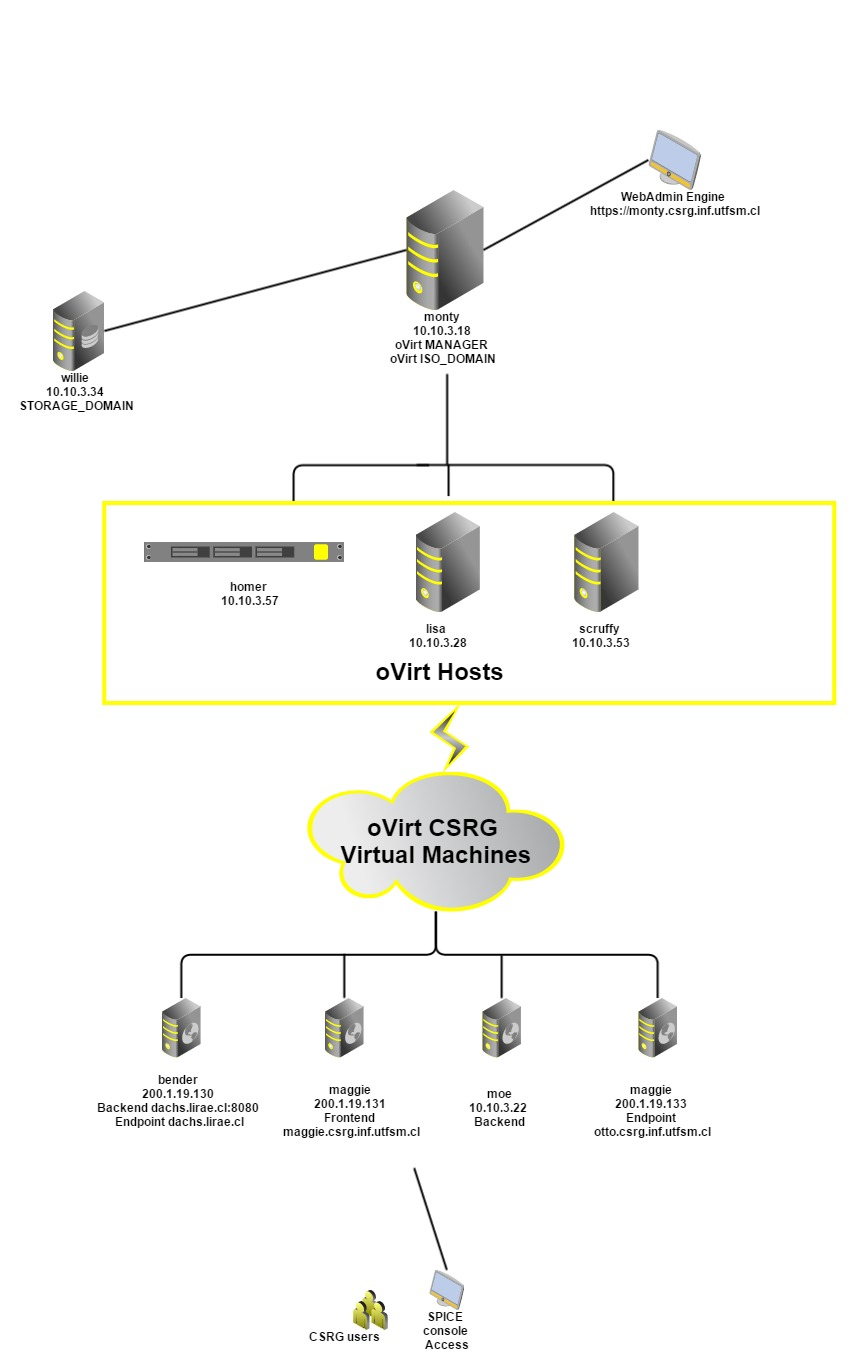
\includegraphics[scale=.21]{img/ovirt}
	\end{center}
	\caption{Esquema de virtualización para ChiVO.}\label{img:ovirt}
\end{figure}
